%
% 1.2
%
\section{Course setup}%
	%
	%
	\label{sec:course-setup}%
	\index{Course!Setup}%
	%
	%
	
	\newthought{This course uses Stata} as its statistical software of choice. Stata is used by many social scientists working with quantitative data in areas such as economics and political science.%
	%
 	\footnote{For example, you will find Stata output in some of Nate Silver's work at the \emph{New York Times} on his `FiveThirtyEight' electoral blog; see, \eg, ``'\href{http://fivethirtyeight.blogs.nytimes.com/2012/03/12/polling-in-deep-south-has-posed-challenges/}{Polling in Deep South Has Posed Challenges},'' 12 March 2012.} %
	%
	Most statistical procedures used in these disciplines know some form of implementation in Stata, and the software is supported by a large user community. It provides a good middle ground between a spreadsheet editor and a statistical programming environment.%
  	
	\newthought{This section} explains how to set up Stata to follow the course. It assumes very little knowledge of computers. \hlred{\textbf{Make sure that you successfully set up your computer} for the course, and that you know how to run the setup again if needed.}%

  \newthought{We will use the `Standard Edition'} (\textsc{se}) of Stata~12 that works on most current computers.%
  \footnote{See the list of Stata products and compatible operating systems: %
		\url{http://www.stata.com/products/compatible-operating-systems/}}%
		%
		The keyboard shortcuts we provide are for \OSX (Mac) and Windows (Win). The installation procedures on both systems are almost identical:% 
		
	\begin{description}

		\item[On \OSX] %
		%
		The entire Stata application folder should be located in the \texttt{Applications} folder. You should drag the Stata application icon to your Dock for quicker access. The \kbd{Cmd} (Command) key used in keyboard shortcuts is the `Apple' modifier key located left and right of the spacebar.%

		\item[On Windows] %
		%
		The entire Stata application folder should be located in the \texttt{Program Files} folder, or whatever your version of Windows calls it. You should drag the Stata application icon to your Taskbar for quicker access. The \kbd{Ctrl} key used in keyboard shortcuts is the `Control' modifier key located bottom-left of the spacebar.%

	\end{description}

	The course runs fine on older versions of Stata. The setup below has been tested on Sciences Po workstations equipped with Stata~11.%
	
	% 0.2.1
	%
	\subsection{Get the teaching material}%
		\label{sec:teaching-pack}%
		\index{Course!Teaching material}

	\newthought{The `Teaching Pack' for this course comes in a single folder,} called the \SRQM folder, which you will have to access very frequently inside and outside class. Download and unzip the folder from its webpage%
		\footnote{\url{http://f.briatte.org/srqm/}} %
		or use the copy provided in class, and keep the \ZIP archive of the folder as a backup.%
		
	\hlred{Move the \SRQM folder to a \textbf{stable location} that you can easily locate on your hard drive, and keep it at that same location throughout the entire course.} Most users deal with this requirement by putting the \SRQM folder with the rest of their study files and then creating an alias to it on their Desktop.%
	
	Use any method that does not involve clicking for two full minutes to access the \SRQM folder, and do not rename its enclosing folders. For simplicity, leave the folder name to \SRQM for the class, and rename it to whatever you like at the end of the semester.%
	
	At that stage, \textbf{check the contents} of the \SRQM folder. The \SRQM folder contains the entire course material, minus the copyrighted textbooks and Stata software. The full contents of that folder, shown in Figure~\ref{fig:srqm-folder}, must stay available on your hard drive during the entire course.%
		%
		%

		\begin{figure}%
		  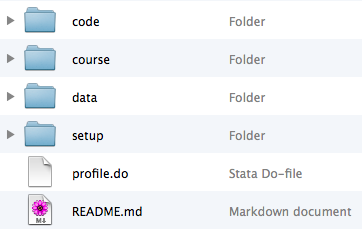
\includegraphics[width=\textwidth]{srqm-folder}
      
		  \caption{The contents of the \SRQM folder should match %
			this screenshot from a \OSX setup.}
		  \label{fig:srqm-folder}
		\end{figure}
		%
		%
		
	The \course folder contains the course slides and syllabus, as well as this guide. The \data folder contains a selection teaching datasets, and the \code folder will host the course do-files (covered below at p.~\pageref{sec:do-files}). The \setup folder and \texttt{profile.do} files provide additional course functionalities. All folders are required for the course to roll out properly.%
		%
		%	\index{Computers!File and folder paths}%

	\index{Computers!URLs}%
	You need to understand the file structure of the course to understand how Stata will locate its files and folders from their \textbf{paths}. The path to the \SRQM folder, for example, might look like this on \OSX:\\[1em]%
	
	\begin{docspec}
		/Users/fr/Documents/Teaching/SRQM
	\end{docspec}
	
	On Windows, the path generally starts on the \texttt{C:} drive and is shown with \texttt{\textbackslash} backslashes:%
		\footnote{Stata for Windows also understand paths with forward slashes.}%
    
	\begin{docspec}
		C:\textbackslash{}Users\textbackslash{}Ivo\textbackslash{}Desktop\textbackslash{}SRQM
	\end{docspec}
	
	On Linux Ubuntu, the path might look something like:%
	
	\begin{docspec}
		\textasciitilde/Joel/Documents/Teaching/SRQM
	\end{docspec}
	
	Once a folder has been set as the \emph{working directory}, Stata can locate files and folders from within it by using relative paths. The example below shows the relative path of the \texttt{nhis2009.dta} dataset in the \texttt{\data} folder:\\[1em]%
	
	\begin{docspec}
		/Users/fr/Documents/Teaching/SRQM/\hlred{\underline{data/nhis2009.dta}}
	\end{docspec}

	File paths are used in Stata to open and save datasets and other types of files. In some cases, it is also possible to open files from online sources by specifying their \URL. A \URL is an Internet address like the one that brings up the course webpage.%
		\footnote{\url{http://f.briatte.org/teaching/quanti/}}%
		%
		%
	
	We will use file paths and URLs extensively throughout the course, so make sure that you understand both. I do my best to keep things tidy on my end by using Internet shortlinks and simple, informative folder and file names for the course material. You will have to do the same on your end.%
		%
		\footnote{For instance, you will be required to submit your work under a specific group name that includes your family names in alphabetical order.}%
		%
		%

	% 0.2.2
	%
	\subsection{Set your working directory}%
		\label{sec:working-directory}%
		\index{Course!Teaching material}

  \newthought{Open the Stata program.} \OSX users can simply double-click the application icon (Figure~\ref{fig:stata-icon}). \hlred{\textbf{Windows users} will have to run Stata with administrator privileges: do this by right-clicking the Stata application icon then selecting `Run as Administrator.'} This will allow Stata to save files anywhere on the hard drive, which is required only for this setup.%

		\begin{marginfigure}
			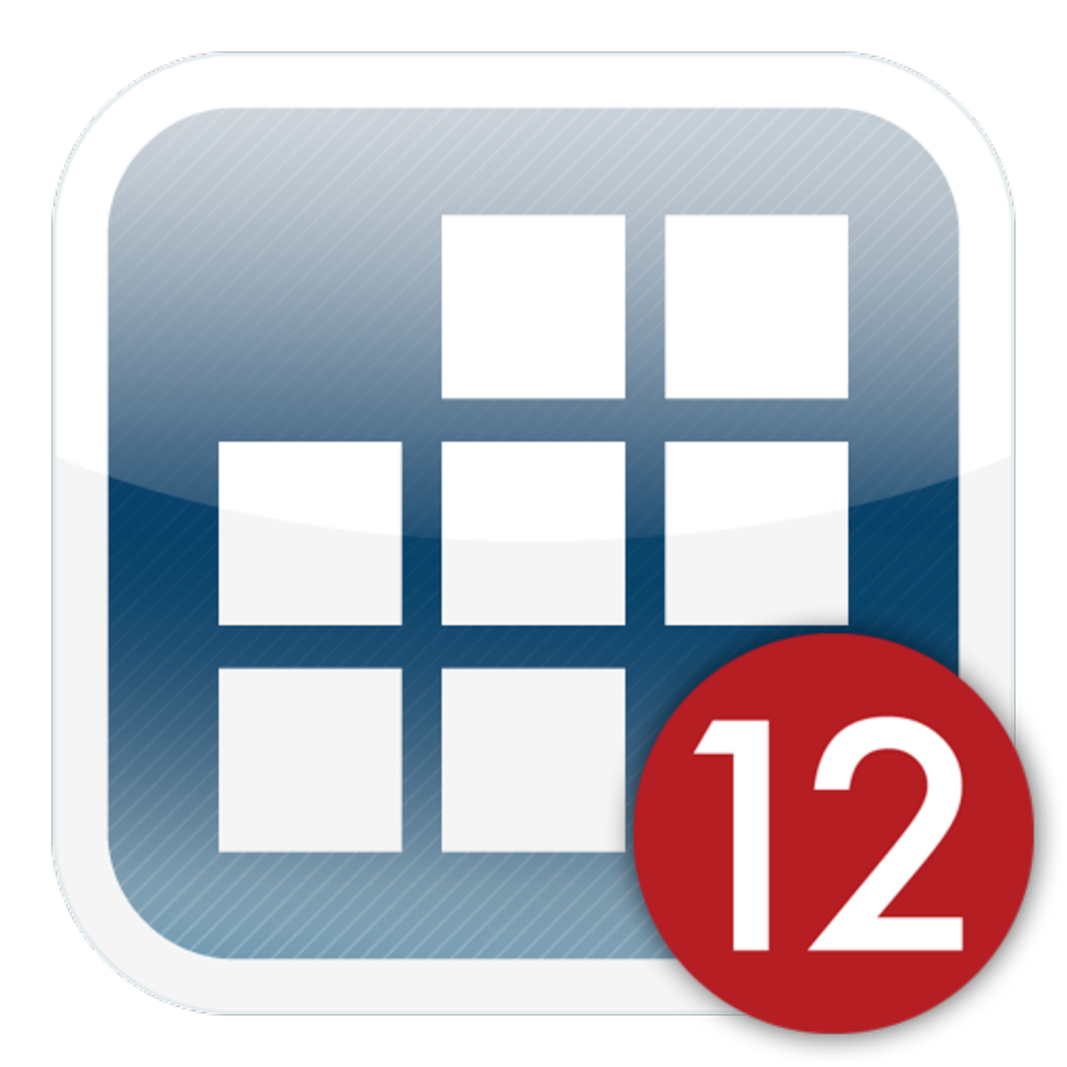
\includegraphics[width=.75\textwidth]{stata-icon}
			\caption{The Stata~12 icon.}
			\label{fig:stata-icon}
	  \end{marginfigure}
	 
	You are now going to set the working directory, which is the folder in which Stata opens and saves files by default. From the `File' menu, choose `Change working directory...', then select the \SRQM folder and press \texttt{Enter}. You will see something like the following printed in the Results window, that is, a folder path ending with the \SRQM folder:\\[1em]%
	
		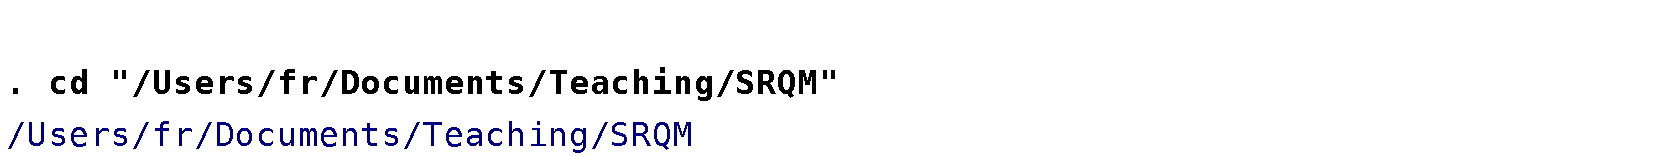
\includegraphics{srqm-cd}\\[1em]

	As the code output shows, the Stata command to do what you did through the `File' menu is \cmd{cd}, for `\underline{c}hoose \underline{d}irectory,' followed by the path to the desired folder. Now that you have learnt a Stata command, try it out by typing the following lines in the Command window and pressing \texttt{Enter} to execute each line:%
	
	\begin{docspec}
		cd ..\\
		cd SRQM
	\end{docspec}
	
	The first command, \texttt{cd ..}, changes the working directory to the enclosing folder, which in my case is the \texttt{Teaching} folder. The second command returns to the \SRQM folder and makes it the working directory again:\\[1em]%
		
	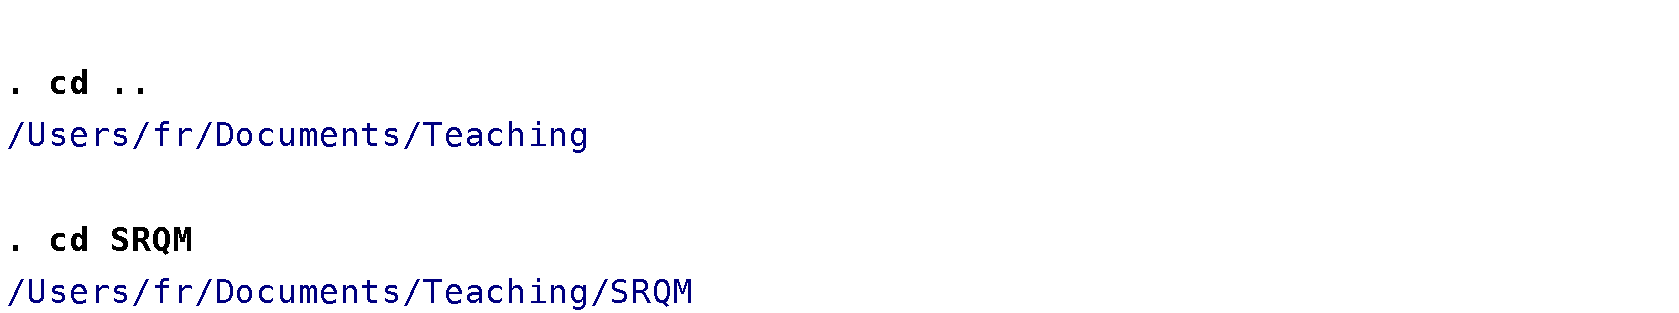
\includegraphics{srqm-cd-back}\\[1em]
	
	You can also list the contents of the working directory with the \cmd{ls} command. The example below will show the full contents of the \SRQM folder with detailed file information:%
	
		\begin{docspec}
			ls
		\end{docspec}

		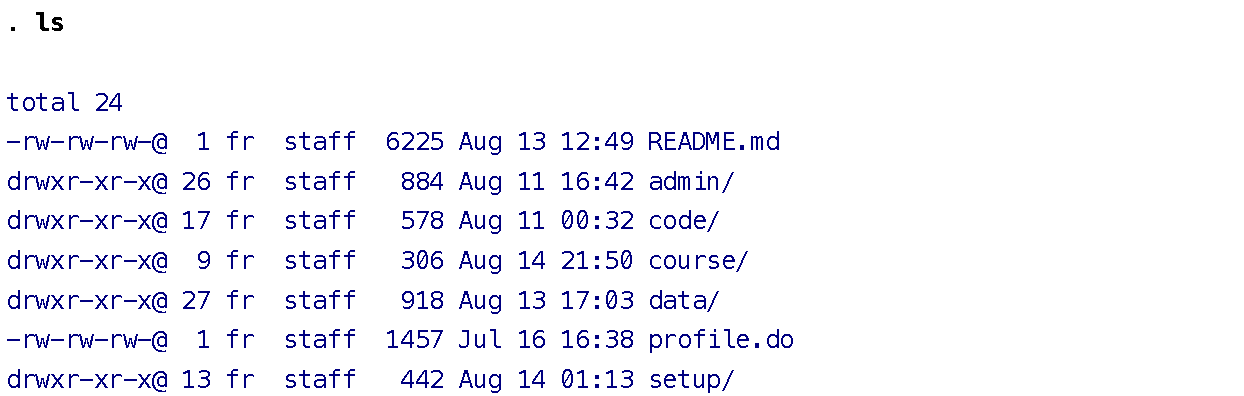
\includegraphics{srqm-ls}\\[1em]
			
	The \cmd{ls} command below will produce a more focused output by listing only the files located in the \data folder that end with the \ext{.dta} extension, which is the Stata dataset format (Figure~\ref{fig:stata-dta}):%

		\begin{marginfigure}
			
\includegraphics[width=.75\textwidth]{stata-dta-icon}
			\caption{Stata~12 dataset icon.}
			\label{fig:stata-dta}
		\end{marginfigure}

		\begin{docspec}
			ls data/*.dta, w
		\end{docspec}
			 
	The command will list the teaching datasets used in the course, for which some documentation is available in the course appendix at p.~\pageref{sec:data-sources}. The \cmd{ls} command is told to only show their filenames by passing the \coab{wide}{w}{ls} option to it:\\[1em]%
 
		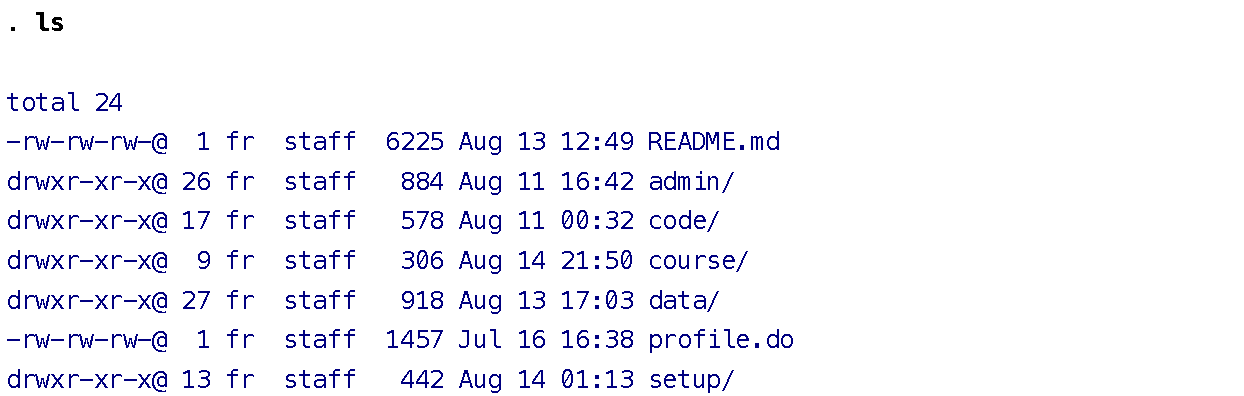
\includegraphics{srqm-ls}\\[1em]
	
	To finish this little exercise with folder navigation from the command line, make sure that your working directory is the \SRQM folder. Use the \cmd{pwd} command to get the path printed once more:%
	
		\begin{docspec}
			pwd
		\end{docspec}
	
	Your working directory should again end with the \SRQM folder, which is what we need to run the course setup in the next section:\\[1em]%
	
		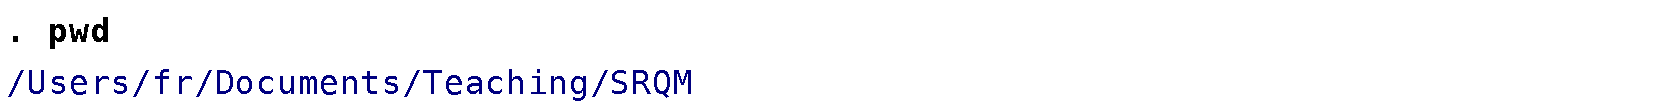
\includegraphics{srqm-pwd}\\[1em]
  
  %
	%
	% 0.2.3
  %
  \subsection{Run the \SRQM setup}%
		\label{sec:setup}%

	To finish setting up your computer for the course, make sure that you are connected to the Internet, then type the following command in the Command window and press \texttt{Enter}:%
		%
		%
		
		\begin{docspec}
			run profile
		\end{docspec}
	
	\hlred{\textbf{Note:} the command will not work if you have not set the \SRQM folder as your working directory}, and that its syntax is a strict one: do not add capital letters, separate the words \texttt{run} and \texttt{profile}, and of course, use the exact spelling.%
	
	This command will trigger a bunch of setup utilities that install the additional Stata commands listed in Table~\ref{tbl:additional-commands}, uncompress the course datasets and adjust some Stata system options.%
		%
		\footnote{For example, the setup adjusts Stata memory on older versions of Stata to deal with some of the larger course datasets. Stata~12 now handles memory automatically.} %
		%
		%
		
	\bigskip
 
  \begin{fullwidth}
		\begin{table}
			\footnotesize
			\begin{tabular}{lll}
			\toprule
			Package & Description \\
			\midrule
			\emph{Installed from the \SSC server:} & & \\
		  \quad \cmd{estout} & export regression results \\
			\quad \cmd{fre} & frequencies with value labels \\
		  \quad \cmd{kountry} & standardised regions and country names\\
		  \quad \cmd{leanout} & simplified regression results\\
			\quad \cmd{lookfor\_all} & search for variables across datasets \\
		  \quad \cmd{mkcorr} & export correlation tables\\
		  \quad \cmd{plotbeta} & regression coefficient plots \\
      \quad \cmd{scheme-burd} & blue-red graph scheme\\
			\quad \cmd{spineplot} & mosaic plots \\
		  \quad \cmd{spmap} & maps\\
		  \quad \cmd{tab\_chi} & residuals for Chi-squared tests\\
		  \quad \cmd{tabout} & export summary statistics\\
		  \quad \cmd{wbopendata} & download World Bank data\\
			\addlinespace
			\emph{Installed from elsewhere:} & & \\
			\quad \label{install-gstd01}\cmd{gstd01} & standardize a variable to $0$-$1$; used at p.~\pageref{sec:gtsd01}\\%
			\quad \label{install-clarify}\cmd{clarify} & simulation\\%; used at p.~\pageref{sec:clarify}\\
			\quad \cmd{schemes} & additional graph schemes\\
			\bottomrule\\[.5em]
			\end{tabular}
			%
			\caption{Additional commands installed by the course setup.}%
			\label{tbl:additional-commands}
		\end{table}
  \end{fullwidth}
  
	You will get a `\texttt{Hello!}' message when the setup is complete.%
	
  \hlred{\textbf{Note:} if you move or rename the \SRQM folder, the setup will break and you will have to repeat the steps covered in the previous paragraphs to fix the issue:}%
		%
		%	
		\begin{enumerate}
			\item run as administrator (if using Windows),
			\item select the \SRQM folder as the working directory, and
			\item type \texttt{run profile} to go through setup again.
		\end{enumerate}
	  
	The setup overwrites the \filename{profile.do} file of the Stata application folder to redirect it to the \SRQM folder for the time of the course. From there, it runs another \filename{profile.do} file that verifies the integrity of the teaching material and reruns parts of the setup if necessary.%
		%
		%
		
	The setup also loads the \cmd{srqm} teaching utilities, like \cmd{srqm\_get}, which is used in class to download the latest version of the course material from a temporary course server, and \cmd{stab}, which is used to produce \underline{s}imple \underline{tab}les of summary statistics (see its detailed instructions at p.~\pageref{cmd:stab}).%
    %
    %
		
  \newthought{At the end of the course}, delete the \texttt{profile.do} from the Stata application folder to stop automatically setting the \SRQM folder as your working directory. Alternately, run the \texttt{srqm\_link, clean} command to do so and get a `\texttt{Bye}' message. This will let you work with Stata from any other working directory.%
		%
		%